\chapter{图论 - 路径和算法}

\begin{figure}[ht]
  \centering
  \includegraphics[width=1\linewidth]{asset/茶桁的 AI 秘籍_Math_25.png}
\end{figure}

\newpage

在充分了解图的概念, 构成以及种类之后, 我们要开始进入稍微有点难度的部分了. 这节课, 咱们来了解一下路径和 Dijkstra 算法. 

\section{拓展: 顶点和边的互换}

在这节课正式开始之前, 我们对上一节课稍微扩充一些内容. 线下有小伙伴问我, 顶点和边的互换问题. 我是没想到会有小伙伴会往深层次去挖, 这样挺好. 

那既然问到了, 我就稍微讲一下. 顶点和边确实是可以互换的, 这代表了更深一层的抽象性. 就比如说图\ref{fig:img26_1}, 它是由这些顶点 ABCDE 以及这几条边构成的. 

\begin{figure}[ht]
  \centering
  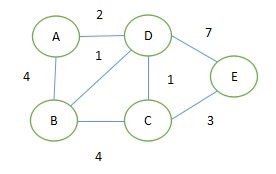
\includegraphics[width=0.5\linewidth]{asset/20230924051221.jpg}
  \caption{}
  \label{fig:img26_1}
\end{figure}

我们也可以把这个边给它重新定义一下, 比如我们把连接 A、D 的这条边在一个新的图里面把它当成一个顶点. 因为虽然说这个图它是由顶点和边构成的, 但是我们在定义它的时候并没有说到它必须得代表什么样的含义, 实际的含义是我们赋予给它的. 所以这里我完全可以用一个新图, 在这个新图里面顶点就代表这些边. 
可以使用数字 1 来表示原来的边为顶点, 然后 A、B 这条边我们用数字 2 来表示. 这里就有两个顶点了. 

之前的 2、4 这两条边都用 A 来链接, 在我们新的图里面就可以类比一下, 就可以把 A 所对应的这个顶点当做我们新图的这个边. 

我们知道边它对应着什么含义, 它是连接了两个顶点. 而在我们这个新图里面, 这个顶点是原来的这个图里面的边. 通过这样的方式去做了一个顶点和边的一个互换. 

本来呢不想说这个, 怕把大家给绕晕. 因为这个是更深一层, 更抽象一点点的这个含义. 所以如果大家能想到这层也非常好啊, 你要知道这个不是什么东西是永恒的, 没有什么东西是永恒的. 

不是这个边它永远是边, 它在另外一个图里面可以是一个结点, 而这个结点在另外一些图里面它可以是一个边. 

\section{最短路径问题}

OK, 让我们回到这节课要讲的内容里. 

在图中, 有一个最短路径问题, 非常的有意思, 也非常重要. 如果你曾学算法数据结构的话, 肯定会遇到这种问题. 我们今天就来探讨一下, 怎么样用图论的思想或者说角度去处理这种问题. 

首先我们有一个赋权图 \ref{fig:img26_2}, 这个图里面它是只对边去做了一个赋值. 这些边都有一个权重, 这些顶点 ABCDE 代表了不同的城市, 权重代表了不同城市间的一个距离. 我给定一个起点, 让你求从这个起点出发, 到剩下的任意一个点的最短路径. 这个要怎么求?

\begin{figure}[ht]
  \centering
  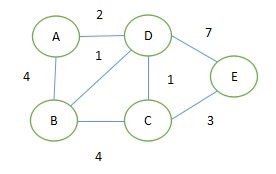
\includegraphics[width=0.5\linewidth]{asset/20230924051221.jpg}
  \caption{}
  \label{fig:img26_2}
\end{figure}

可能如果是用肉眼去观察的话, 在这个图的结点数以及这个边数不是很多的时候我们看也能看出答案. 但是这个不是我们一个终极意义, 我们的一个终极意义是希望找到一种自动化的过程. 不管这个顶点数量有多少, 边的数量有多少, 都希望能让计算机按照我规定的方式去找到最短路径. 希望找到解决这一类办法的一个通解. 

所以问题来了, 就是如果我们是 A 点出发的话, 怎样去求到剩下的 BCDE 各个点的一个最短路径呢?从 A 到 B, 他们俩确实直接相连的, 他这个 A、B 边的权重是 4, 但我们会发现如果通过 D 来中转一下,A、D 是 2, B、D 是 1,  2+1 等于 3, 它是小于 4 的. 

所以在这个时候可能它最短路径不是 A、B 直接相连的这条边, 可能更好的选择是走 D 绕一下路. 对于这种比较复杂的情况, 我们应该怎么样去找?

\section{Dijkstra 算法}

对于上面所提出的最短路径问题, 就需要提出一个算法了, 就是我们的 Dijkstra 算法. Dijkstra 算法是解决这种路线规划问题, 最短路线问题非常有效的一种方法. 

他的思路就是, 首先我们先把顶点的集合 V 给分成两组, 一组是 S, 一组是 U. 

S 是已解决的顶点的集合, 初始时只含有源点 V0. 已解决就是从起点出发到 S 集合里面这些顶点的最短路径已经被求出来了, 这些点的我们称之为已解决. 

U 是我们还未确定的顶点集合. 

将 U 中顶点按递增的次序加入道 S 中, 保证下面两点: 

\begin{itemize}
  \item 从源点 V0 到 S 中其他各顶点的长度都不大于从 V0 到 U 中任何顶点的最短路径长度. 
  \item 每个顶点对应一个距离值
\end{itemize}

定义好之后, 初始的时候我们只有这个起点, 人是待在起点的, 还是一个待出发的状态. 所以一开始 S 这个集合里面只有 V0 这个点, 在图里面它就是 A. 接下来, 我们先看这个 U,U 中的顶点是按照递增的次序加入到 S 中, 也就是初始化的时候, 虽然这些 U 还是没有被解决, 但是在一开始的时候也赋予了 U 中的点到原点的一个初始距离. 

比如一开始的时候原点是连接了所有的这个顶点的, 这种情况下它就有一个初始值, 我们就按照这种初始值从小到大排列. 每一次去取一个在 U 当中和这个原点距离最短的那一个点出来. 

然后我们保证这个原点 V0 到 S 是不大于从 V0 到 U 中的任意一个点. 

S 当中包含已经找到最短路径的点, 要确保 U 中不存在中转点, 使得从 V0 到这些中转点, 再从中转点到 S 里其他的一些点的距离比通过它这个中转要长. 

S 中顶点: 从 V0 到此顶点的长度
U 中顶点: 从 V0 到此顶点的只包括 S 中顶点作中间顶点的最短路径长度. 

每个顶点都对应一个距离值,这个距离值就是目前当下从起点 V0 到顶点所对应的一个最短距离. 

当然还有一点就是 S 中的顶点, 比如 V1 这个路径, 不一定是从 V0 直接到 V1 的, 可能是通过 S 中的其他点中转, 然后再到 V1. V0 先到 V2, 然后再从 V2 到 V1, 这是我们找到一个从 V0 到 V1 的一个最短路径. 它不一定是直接的, 这点大家要注意. 

S 中的顶点, 这个距离值是什么呢?刚才说了, 每个顶点都对应了一个距离值. S 中的这个顶点对应的距离值和 U 中的顶点对应的距离值是不太一样的. 

S 中的顶点就是代表了从 V0 到这个点的最短路径的一个长度. 就是最短路径已经找出来了, 不管是 V0 直接到 V1, 还是 V0 通过中转其他点到 V1 的, 总之最短距离是找着了. 

U 中的顶点是从 V0 到这个顶点, 包括在 S 中的顶点作为中转点的一个最短路线. 

比方说, S 中已经有 V0、V1 这两个点了, 现在 U 中有 V2、V3. U 中的这个 V2 对应的这个距离是什么意思呢?要么就是 V0 直接到 V2, 有个直飞航班, 要么就是 V0 中转到 V1, 从 V1 到达了 V2. 

所以 U 中这些顶点对应的距离值如果有中转点的话, 中转点一定是属于 S 当中的. 

这就是 Dijkstra 算法的一个思路. 如果单纯看这个步骤会非常晕, 我们接下来看一下这个分步拆解是怎么样做的, 如图\ref{fig:img26_3}. 

\begin{figure}[ht]
  \centering
  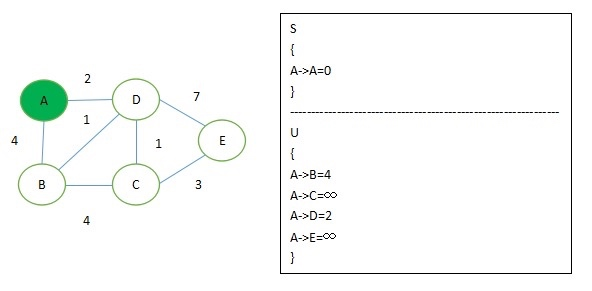
\includegraphics[width=0.7\linewidth]{asset/20230924051222.jpg}
  \caption{}
  \label{fig:img26_3}
\end{figure}

首先这里有两个集合, S 和 U.  S 呢是已解决的, U 是还没有找到最短路径的这些点. 

当然, 这里没有单纯的是用一个点表示, 我们是用这些距离来表示. 但是大家如果要看点的话看第二个, 就箭头指向的是第二个. 

虽然表示的都是距离, 也可以表示点. 比如 A->B, 距离 4 其实针对的是 B 这一点, 我们刚才说了 S 和 U 是顶点的集合. 

有的人可能看到这里会有点晕, 所以我就说一下, 这里虽然写成了距离的形式, 但是他在表示距离的同时也可以代表距离对应的是哪一个点. 

我们一开始的时候就说到了 S 集合里面只有起点, 这里起点是 A, 所以 A 到 A 距离就是 0. 在起点都不用走就已经到了, 所以距离是 0. 

在这里插一点, 就是 S 一开始初始化的时候是只有包含 A 这个点. 而且因为它是起点, 所以 A 到 A 的距离就是 0, 这个很好理解. U 里面的点, 比如说 A 到 B, A 到 D, A 到 C, A 到 E 这些距离, 一般是全部初始化正无穷. 

这里 A 到 B 等于 4, A 到 D 等于 2 是因为 A 可以直接到达两个点 B 和 D, 现在有一个距离 4. A、B 之间本来的距离是正无穷, 现在我们已经找着了, A 可以直接到 B, 它有一个路径是是 4, 所以 4 就取代了正无穷. 因为它是一个更短的路径, 4 是远小于正无穷的, 所以这里用 4 来取代. 大家要注意在初始化的时候 U 里面的 4 个长度全部都是正无穷. 

然后再看, 由 A 可以直接到哪一些点. 和 A 直接相连的, 是 B 和 D 两个点, B 和 D 是和 A 直接相连的, 我们就把 A、D 之间的这个距离, 这个权重和它原来的这个距离正无穷相比, 我们更新了一下数值. 

我们现在知道, 从 A 到 B 的距离不再是正无穷了, 它是 4. 就是 AB 边的权重为 4. 这里 A、D 这个距离是 2, 不再是正无穷了;C 和 E 呢, 因为 A 不是直接相连 C 和 E 的, 所以我们还是把它写成正无穷的形式. 

这就是第一步. 接下来, 我们来看一下在 U 的集合里面边长最短的是哪一条边. 是 AD, 所以我们就把 D 这一点给它再摘出来. 因为它距离最短, 2、4、正无穷、正无穷, 2 是最短的. 我们把 D 摘出来. 

第二步, D 的这个距离最短距离就是 2, 那好, D 的最短距离就是 2, 图\ref{fig:img26_4}. 

\begin{figure}[ht]
  \centering
  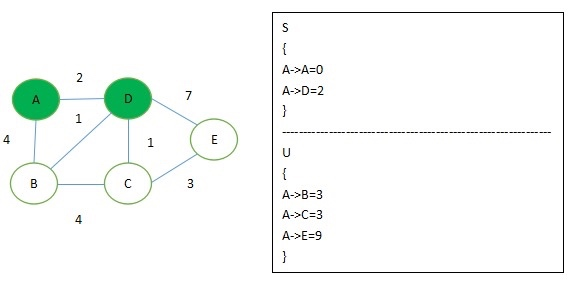
\includegraphics[width=0.7\linewidth]{asset/20230924051223.jpg}
  \caption{}
  \label{fig:img26_4}
\end{figure}

接下来我们就要更新 BCE 的距离了. 很巧的是 BCE 三点都和 D 直接相连. 我们现在来做一个什么样的判断呢?先来看一下到 B 点, 原本 A 到 B 的距离我们在上一步是求出来的, 在上一步当中它最短的距离直航航班. A 到 B, 权重 4, AB 在上一步里面是 4. 

接下来 D 已经是放在 S 里面, 然后从起点 A 出发到 D 的最短距离已经确定了是 2. 所以我们现在就来看从 A 到 D 的这一部分路程, 再加上 D 到 B 的这个路程会不会比上一步得到的 AB, 也就是现在得到的 AB 直行的路程要短. 一加发现 2+1=3 是小于 4 的, 所以在这步里面呢我们就把 A 到 B 的距离给它更新一下, 就由 4 更新成了 3. 

同理, 我们再来看一下 AC, 在上一步我们知道它本来是正无穷, 因为我们在上一步没法更新, A 和 C 不直接相连, 所以还是初始化里面的那个正无穷. 现在 D 我们可以处理它, 因为 D 有直飞航班可以到 C, 所以我们做同样的一个判断, 就是 A 到 D 的距离再加上 D 到 C 的距离会不会比上一步得到的 AC 的距离要小?结果是确实小,$ 2+1=3$小与正无穷. 在这里 A 到 C 的距离也被更新了, 更新成 3. 

接下来再看 E, 我们在上一步也知道 AE 本来还是初始化的正无穷. 因为 A 没法到 E, 所以上一步判断不了, 就只能暂且保留初始化值. 

接下来我们可以去探索了, 因为 D 也有直飞 E 的航班, 所以我们来看一下, A 到 D, 然后 D 到 E 这两段路程加在一块会不会比上一步的从 A 到 E 的距离要短?$2+7=9$, 9 小于正无穷, A 到 E, 我们这个距离也从正无穷更新成了 9.

好, D 也就处理完了, 和它相邻的这 BCE 三个点我们都已经处理完了, 所以就不用去看了. 接下来再看 U 里面还剩哪三个点, 分别是 BCE. 

BCE, 我们看哪一个点对应的距离在 U 里面当下是最小的?而这里有两个相等的, AB 是 3, AC 也是 3. 这个都无所谓, 我们任选一个都 OK. 我们就选 B, 选了 B 之后, 我们知道 AB 通过上一步的判断, 最短路径是通过 D 来中转了一下, 然后到达了 B. 所以 AB 在这里已经确定的最短路径不是从 A 直接到 B, 而是我们从这个 A 转 D 再到了 B. 这个 B 到起点的距离也已经确定了, 就是 3. 之后起点到 B 这个距离就不再是 4 了. 按照最短路径找到的结果, 就按 3 来计算, \ref{fig:img26_5}. 

\begin{figure}[ht]
  \centering
  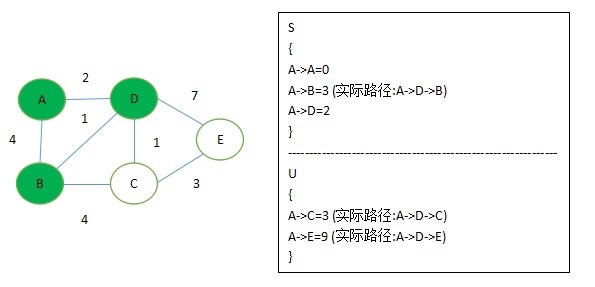
\includegraphics[width=0.7\linewidth]{asset/20230924051224.jpg}
  \caption{}
  \label{fig:img26_5}
\end{figure}

然后我们把 B 拎出来, 看 B 还和 U 当中的哪一个点有直接的联系, 就是有边相连. 那就是 C 了. 

C 在上一步得到的结论是由 A 中转 D 再到 C 的距离仅仅是 3, 那我们来看, 现在尝试着从 B 中转到 C, 能不能让这个距离更缩短一点. 结果 A 到 B 要花费 4, B 到 C 又是 4, 所以 4+4=8, 它是大于 3 的, 没有上一步那个解更优. 所以这个值还是保留下来了, 不做更新. 

然后是 E, 因为 B 和 E 不直接相连, E 也没有去做更新, 那接下来我们再重复之前的一个步骤. 

挑出来 A 到 C 等于 3, 这个是已经确定了一个最短路径, 然后我们把这个 C 点给摘出来, 就进入我们的下一步, \ref{fig:img26_6}. 

\begin{figure}[ht]
  \centering
  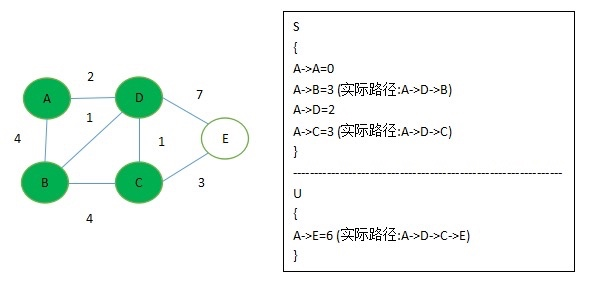
\includegraphics[width=0.7\linewidth]{asset/20230924051225.jpg}
  \caption{}
  \label{fig:img26_6}
\end{figure}

进入到下一步之后, C 到起点 A 的这个最短路径都已经确定了, 接下来再看一下 U 当中和 C 相连的点只剩哪一个了?只有 E 了对吧,U 当中只有一个 E 了,也就是我们可以把 E 也当做一个终点. 

之前我们讨论过 A 到 E, 它是从 D 中转的. 先由 A 到 D, 然后由 D 到 E, 这是我们在判断 D 这个点的时候判断出来一个结果. 在那一步我们确定了 E 到 A 的最短距离是经 D 中转也就是$2+7=9$. 

我们现在再探讨点 C, 能不能通过 C 点这个中转, 让 A 到 E 的距离更短呢?我们会发现 A 到 C 的距离是判断出来了, 是走 D 中转, 所以是 ADC. 从 A 到 C 的距离, 再加上 C 到 E 的距离, 2+1+3=6, 6 是小于 9 的. 所以我们也就把最后这一个点给更新了. 

在这里 A 到 E 的这条路径就是由 9 更新成了 6. 它的实际路径是 ADCE. \ref{fig:img26_7} 

\begin{figure}[ht]
  \centering
  \caption{}
  \label{fig:img26_7}
  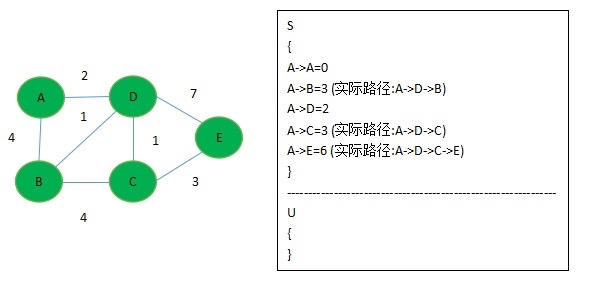
\includegraphics[width=0.7\linewidth]{asset/20230924051226.jpg}
\end{figure}

至此为止我们就把所有的点都给它遍历一遍, 已经找出来了. 所以我们在这里就是找到了各个点到起点 A 的一个最短路径, 最短距离. 

当然了, 这个过程我不知道大家如果看每一步这个图解是不是会清楚很多. 如果单纯看那个算法思想确实复杂一点. 这个每一步的图解其实还是很容易理解的. 而且我们在实际操作当中, 也会弄一个数组. 

我们放在 S 中的这每一个点, 不光记录它到起点的最短路径, 还要记住这个最短路径上一个点或者说负结点是哪一个点. 

我们用一个数组去记录下来, 记录下来之后就会发现, C 点的负结点是 D. 然后那我们再来看 D, 它的这个负结点就是 A. 

那为什么要记录这些负结点呢?就是最后要求最短路径, 往往并不是让你直接求出这个距离, 求距离也许很简单, 我是希望能告诉我从 A 点出发经过哪些点到 e. 只要我们能把每一个点放到 S 集合的同时, 把它的这个负结点给记录下来, 每一个点只需要记录它的负结点, 一个跟一个, 我们就可以把整个最短路径给找出来了. 

就像我们以前在中学排队的时候, 体育老师可能说过我们只要记住我们前面是谁
就行了. 前面是小张还是小王, 你就记住你前面一个人就行了, 其他你不用管. 那大家最终都能把这个队列给找出来. 

在这里其实也是一样的, 就是这个目的. 当我们把每一个点放进 S 集合的同时, 我们把负结点也放进最短路径的集合的时候, 是由哪个点到达这个点的这个负结点给它记下来, 我们就能反向推导出来. 

比如, E 点, 我们记录下来它负结点是 C, C 的负结点是 D, D 的负结点是 A. 所以 ECDA, 再把它颠倒过来就是 ADCE. 这个最短路径就找出来了. 这个最短距离也就求出来了. 

我们来看一段动图演示: 动图在 PDF 内不好展示, 可以\href{https://raw.githubusercontent.com/hivandu/notes/main/img/20230924051227.gif}{点击连接看原图}

这个过程其实和我刚才说的是一模一样的, 大家会注意红色的正无穷就代表了我们目前假设的从这个起点到这些点的一个距离的初始化的时候. 全部初始化成了正无穷. 

然后再根据每一步的判断, 不断的把这些点从 U 集合放到 S 集合里面, 然后以你放的点作为一个中转点, 就像一个跳板一样. 

你看哪些点是和你刚放入 S 中集合的点相连, 再看一下通过你刚放的这个点中转能不能让其他的点到起点的距离更短, 就不断的达到更新的效果. 

这个动图大家如果觉得比较快, 可以在此处下载稍微慢速一些的, 因为网站限制无法上传过多帧的动图. 还可以回看一下刚才每一步的一个详解. 

当然, Dijkstra 算法也有一些不太适用的情况. 就是权重如果是有一个负的情况出现的话, 那这个算法它就没办法起到作用了. 

为什么呢?你比如说, 我要求这个 A 点到 B 点的一个最短路径, 我们会发现它有一个直飞航班, 从 A 到 B 的. \ref{fig:img26_9}. 

\begin{figure}[ht]
  \centering
  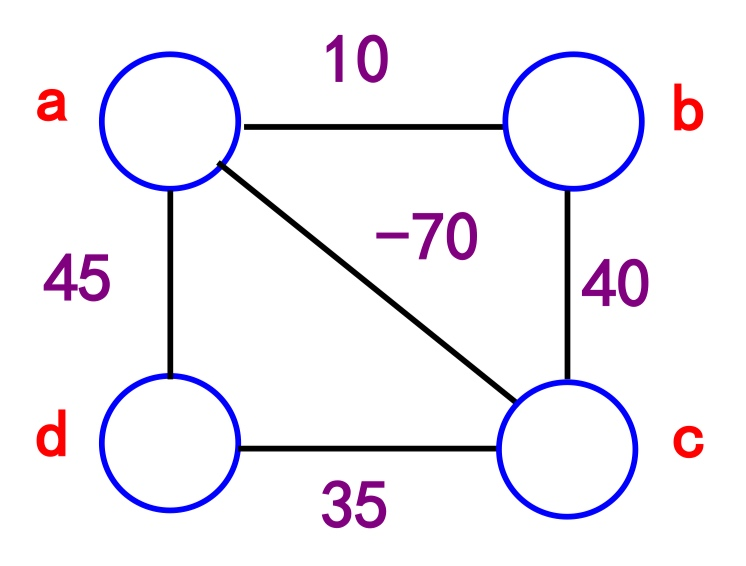
\includegraphics[width=0.4\linewidth]{asset/20230924051228.jpg}
  \caption{}
  \label{fig:img26_9}
\end{figure}

这个权重是 10, 但是我发现如果从 a 到 c 中转一下它变成了-70, 然后从 c 到 b 是 40. 通过这种方式我们去走的话, 通过 C 中转, 这个路程就是-30. 而且这还不算完, -30, 我们再想一下, 这个-30 我们是从 a 到 b, 那我现在从 b 再回到 a, $-30+10=-20$. 但是没关系, 我们再做一次这个循环, 就会发现从 a 到 b 的这个距离会越来越小. 

所以大家要记住, 在这里 Dijkstra 算法如果权重是一个负的情况的话, 他是不太适用的. 尤其是当你形成了这么一个圆圈, 在这个圈里面, 你只要循环一次就能这两个点之间的距离变小. 那你循环无限次, 它距离就能无限变小了. 这个是很显然不符合现实情况的. 这是一个需要大家注意的一个地方. 

好, 那到这里, 我们包括用最短路径问题引出了 Dijkstra 算法, 介绍了其思想和过程, 并且用它演示了一遍求最短路径的经过. 

下一节课, 是我们图论的最后一节课, 也是我们整个「人工智能数学篇」的最后一节课, 我们下一节课会来学习「树」, 了解一下最小生成树. 最后总结一下. 

不过不用觉得遗憾, 因为数学篇只是我们长征路上的一个起点, 我们现在完成了 Python 以及数学基础, 就要正式迈入人工智能的大门了. 